\chapter{MASSIVE Language}
\label{usecase}

In this report we illustrate how we design and implement the agent oriented language, MASSIVE. During this chapter we demonstrate a working simulation with a use case, and compare the agent oriented language to object oriented code (C\#). Furthermore we discuss the advantages and disadvantages of the MASSIVE language. 

\section{Use Case}
This use case demonstrates how to write a wargame scenario in the MASSIVE language, how to compile it, and how to run it. \\
%In this use case we demonstrate how to write a mini-game in our language, how to compile it and how to play it. \\
 \\
The first thing to do is to write the MASSIVE code for creating the agents and alike. In the example two teams are created, these teams are called "Disco" and "Kman". Agents are added to each team and an action pattern is defined, for later use when running the wargame simulation.

\begin{source}{MASSIVE code example}{}

/* Initializes the game */
Main ()
{	
	
	// Creates team Disco.
	new team teamDisco("Disco", "#FF6600");
	num totalDiscos = 10;
	for ( num i = 0; i < totalDiscos; i = i + 1)
	{
		num a = 0;
		if ( i < totalDiscos-1 )
		{
			a = 1;
		}
		else
		{
			a = 21-totalDiscos;
		}
		
		new Agent newAgent("Stue", a);
		teamDisco.add(newAgent);
	}
	
	new team teamKman("Kman", "#660000");
	new squad squadNabs("noobs");
	new squad squadRevo("Revolution");
	
	for(num i = 0; i < 4; i = i + 1)
	{
		num a = 0;
		if(i =< 1)
		{
			a = 2;
		}
		if(i >= 2)
		{
			a = 8;
		}
		
		new Agent newAgent("Kman", a);
		teamKman.add(newAgent);
		
		if (i <= 1)
		{
			squadNabs.add(newAgent);
		}
		if (i => 2)
		{
			squadRevo.add(newAgent);
		}
	}
	
	// Moves used in the actionPatterns.
	string moveUp = "unit move up";
	string moveDown = "unit move down";
	string moveLeft = "unit move left";
	string moveRight = "unit move right";
	
	// Creates the action pattern Patrol Low.
	// Patrols the lower part of the game area.
	new actionpattern patrolLow("PatrolLow");
	patrolLow.add(moveUp);
	patrolLow.add("unit move 25,24");
	patrolLow.add(moveUp);
	patrolLow.add("unit move 0,23");
	patrolLow.add(moveDown);
	
}
\end{source}

When compiling the code the compiler warns that there are unused variables (see \ref{fig:compiler}). This will not produce any fatal compilation errors, but it is just a notification to the programmer. However if any fatal errors are found while compiling the MASSIVE compiler will break the compilation and print the errors.

%We will disregard this for the purpose of this use case, however, if there were serious faults in the code the compiler would warn you the same manner and maybe even refuse to compile if the faults were serious enough.

\begin{figure}[h]%
\begin{center}
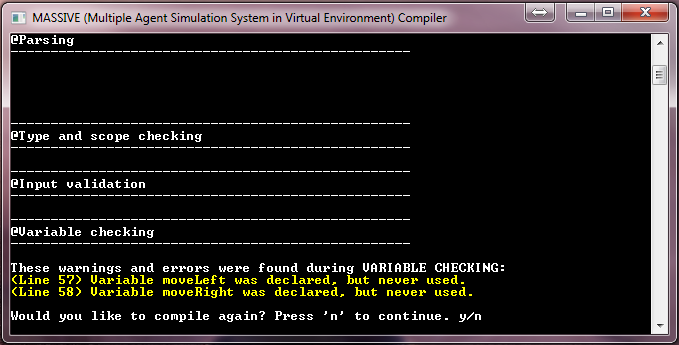
\includegraphics[scale=0.6]{Images/compiler.png}%
\end{center}
\caption{The MASSIVE compiler warning of unused variables.}%
\label{fig:compiler}%
\end{figure}

The MASSIVE compiler provides the programmer with the oppurtunity to recompile the code, which provides the programmer with a way of correcting code containing errors without terminating the compiler everytime it fails. After a succesfull compilation a file named "MASSIVECode.cs" is created. The purpose of creating the .cs file is to be able to compile it with the help of the C\# compiler. The compilation of the .cs file generates an .exe file, which create the actual data output in XML format. The XML-data is then loaded by the MASSIVE battlefield application. When running the MASSIVE battlefield application, the user is given the choice to determin the grid size \ref{fig:game_promt}).

\begin{figure}[h]%
\begin{center}
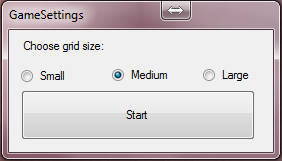
\includegraphics[scale=0.6]{images/massive_dialog.png}%
\end{center}
\caption{Choosing the size of the game-grid}%
\label{fig:game_promt}%
\end{figure}

The user will be presented with the actual simulation (see \ref{fig:runninggame}). Here the user will have the oppertunity to instruct the agents to use the action pattern defined in the previous code example or any of the movement commands, as shown in \ref{fig:runninggame}.

\begin{figure}[h]%
\begin{center}
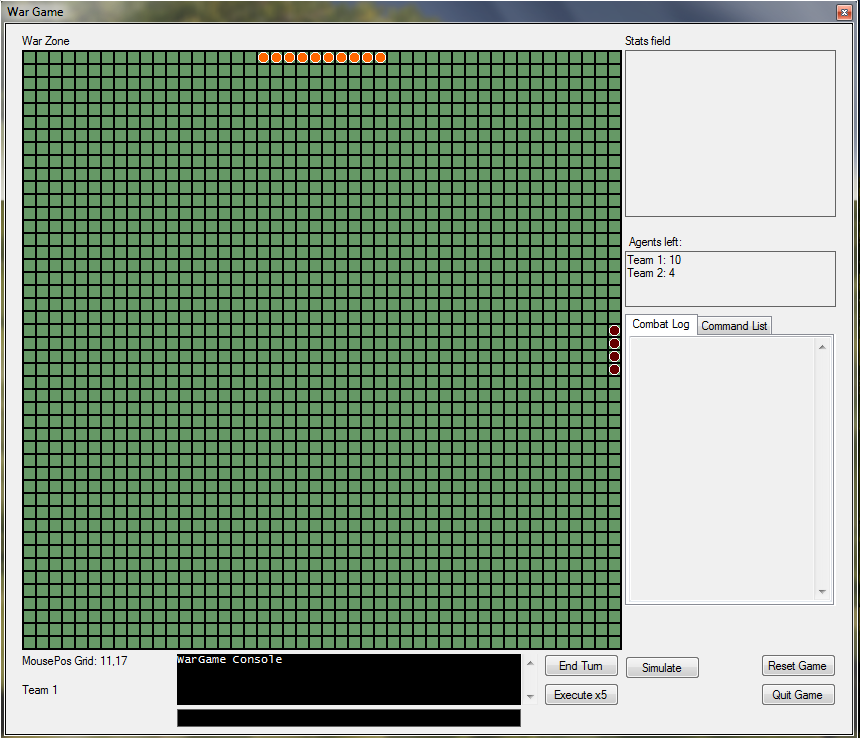
\includegraphics[scale=0.6]{Images/massive_small.png}%
\end{center}
\caption{The simulation running with the input instructing som of the agents to use an actionpattern}%
\label{fig:runninggame}%
\end{figure}

When the MASSIVE battlefield application is running, the user is able to either give commands to the agents, end the current teams turn, run 5 sequal turns, or simulate the wargame untill a winner is found. The figure \ref{fig:winner} is the result of the command "team 2 move patrolLow" followed by an "Execute x5".
%At this point the user is presented with a choice; the "Simulate" button simulates the wargame untill a winner is found, or he can choose to run the game turn-by-turn and control the agents as the game progresses. We see the result of this simulation in \ref{fig:winner}.

\begin{figure}[h]%
\begin{center}
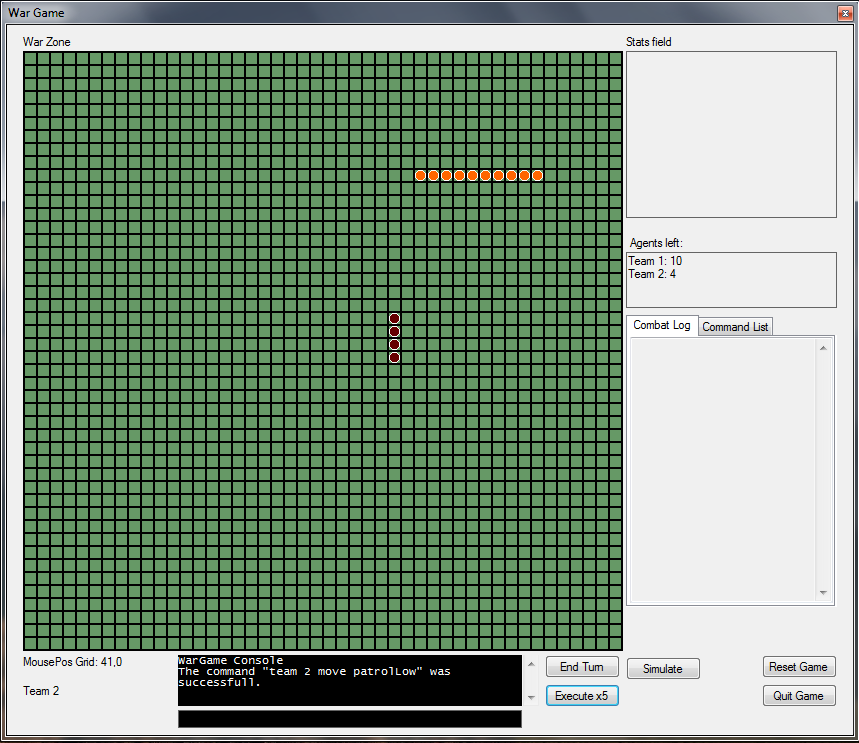
\includegraphics[scale=0.6]{Images/massive_patrollow.png}%
\end{center}
\caption{The result of the command "team 2 move patrolLow" followed by an "Execute x5".}%
\label{fig:winner}%
\end{figure}

\section{Comparison}
\indent This section compares how a wargame can be build using C\# or by using the MASSIVE compiler. We will take a look at some of the pros and cons by using C\#  aswell as the pros and cons using the MASSIVE language.

\section{C\#}
The MASSIVE language is being compared to C\# which is an object orientated language. This was done due to both the compiler and the GUI is written in C\#. C\# does not have a built in multi agent orientated function or enviroment, which means it is required for the programmer to build the multi agent wargame from scratch. Building a multi agent wargame in C\# would require the programmer to have programming knowledge, in the MASSIVE language there are less features, which should make it more simple for first time users.\\
%To build a multi agent wargame in C\# one needs to make constructors for agent and teams, furthermore one also needs to create functions for agents and teams i.e. movements and attack functions.\\

Pros
\begin{itemize}
	\item No limits, you can create all the features you want.\\
\end{itemize}

Cons
\begin{itemize}
	\item No existing multi agent enviroment.
	\item No existing multi agent types.
	\item No existing multi agent functions.
\end{itemize}

\section{MASSIVE}
MASSIVE is a agent orientated language, which contains premade enviroment and functions for creating agents, squads, teams, and actionpatterns, which means that one does not have to build these functions themselves and it is therefore simpler to simulate a wargame in. The MASSIVE language does not support functions, therefore limiting the programmer to use the build in functions. As the MASSIVE language is case insensitive the programmer does not have to think about writing in upper or lower case characters.

%You cannot declare new functions in MASSIVE which limit you to only use the built in functions. The types and functions of MASSIVE are not case sensitve, so you do not need to worry about writing in upper or lower case.\\

Pros
\begin{itemize}
	\item Simple to simulate a wargame.
  \item	Premade enviroment.
	\item Premade types for agent, squad, team, and actionpattern.
	\item The language is case insensitive.
\end{itemize}

Cons
\begin{itemize}
	\item Limited to use build-in functions.
\end{itemize}

%Good and abd things about MASSIVE
%Why is our MASSIVE better than OOP. 
\section{C\# vs MASSIVE}
If the previous MASSIVE code example \ref{usecase} was written in C\# the differences would be how to delcare objects, use num instead of any number denoters, and that the language is case insensitive. Furthermore you cannot increment a number by using "++", but the programmer have to use an assignment instead.
Therefore the most important difference between C\# and the MASSIVE language is, that the MASSIVE language already have build-in types and functions needed by the programmer to initialize a wargame scenario.\\
\\
Below is a comparison between some of the MASSIVE languages functions and the same functions written in C\#. It is implicit that in the C\# examples the types have been created already.\\

%Old code examples
\begin{source}{MASSIVE ActionPattern code example}{}                    
	Main
	{
	new ActionPattern ap("FirstAction");
	ap.add("unit move up");
	ap.add("unit move left");
	ap.add("unit move up");
	}
\end{source}

\begin{source}{C\# ActionPattern code example}{}                    
static void Main(string[] args)
    {
        ActionPattern AP = new ActionPattern("FirstAction");
				ap.add("unit move up");
				ap.add("unit move left");
				ap.add("unit move up");
    }
\end{source}

A noticeable difference is that the programmer does not have to write the long definition to initialize the main method and ActionPattern is only written once to be declared.


\begin{source}{MASSIVE Teams code example}{}                    
	Main
	{
		new team teamDisco("Disco", "#FF6600");
		new team teamKman("Kman", "#660000");
	}
\end{source}

\begin{source}{C\# Teams code example}{}                    
	static void Main(string[] args)
    {
        Team teamDisco = new Team("Disco", "#FF6600");
				Team teamKman = new Team("Kman", "#660000");
    }
\end{source}

Again the programmer dont have to write as much code, because the MASSIVE language does not require that the programmer is able to write object oriented types and objects.
